\documentclass{article}
\usepackage{amsmath, amssymb, cite, algorithmic, url, braket}
\usepackage{graphicx}
\usepackage{pythonhighlight}
\usepackage[margin=1.5cm]{geometry}
\usepackage[title]{appendix}
\usepackage{subfigure}
\usepackage{listings}
\usepackage{booktabs}

\graphicspath{{../pic/}}
\lstset{
language=[ANSI]{C},
showtabs=true,
tab=,
tabsize=2,
basicstyle=\ttfamily\footnotesize,%\setstretch{.5},
stringstyle=\color{stringcolour},
showstringspaces=false,
alsoletter={1234567890},
otherkeywords={\%, \}, \{, \&, \|},
keywordstyle=\color{keywordcolour}\bfseries,
upquote=true,
morecomment=[s]{/*}{*/},
commentstyle=\color{commentcolour}\slshape,
literate=*%
{=}{{\literatecolour=}}{1}%
{-}{{\literatecolour-}}{1}%
{+}{{\literatecolour+}}{1}%
{*}{{\literatecolour*}}{1}%
{!}{{\literatecolour!}}{1}%
{[}{{\literatecolour[}}{1}%
{]}{{\literatecolour]}}{1}%
{<}{{\literatecolour<}}{1}%
{>}{{\literatecolour>}}{1}%
% {>>>}{\pythonprompt}{3}%
,%
frame=trbl,
rulecolor=\color{black!40},
backgroundcolor=\color{white},
breakindent=.5\textwidth,frame=single,breaklines=true
}

\begin{document}
\title{DSP Homework 12}
\author{Xu, Minhuan}
\maketitle
\tableofcontents
\begin{abstract}

\end{abstract}

\section{Videos}

\section{Frequency Range of Voice}
To find the range of my voice frequency, I want to record my voice and do FFT to it. Then, I filter some frequencies under or beyond a certain value, if I can hear my voice, I filter more frequencies out until I cannot hear my voice. See Fig.~\ref{fig:voiceSpectrum}, there are the original wave, wave through a high-pass filter and spectrum of the 2nd wave.

\begin{figure}[!h]
	\centering
	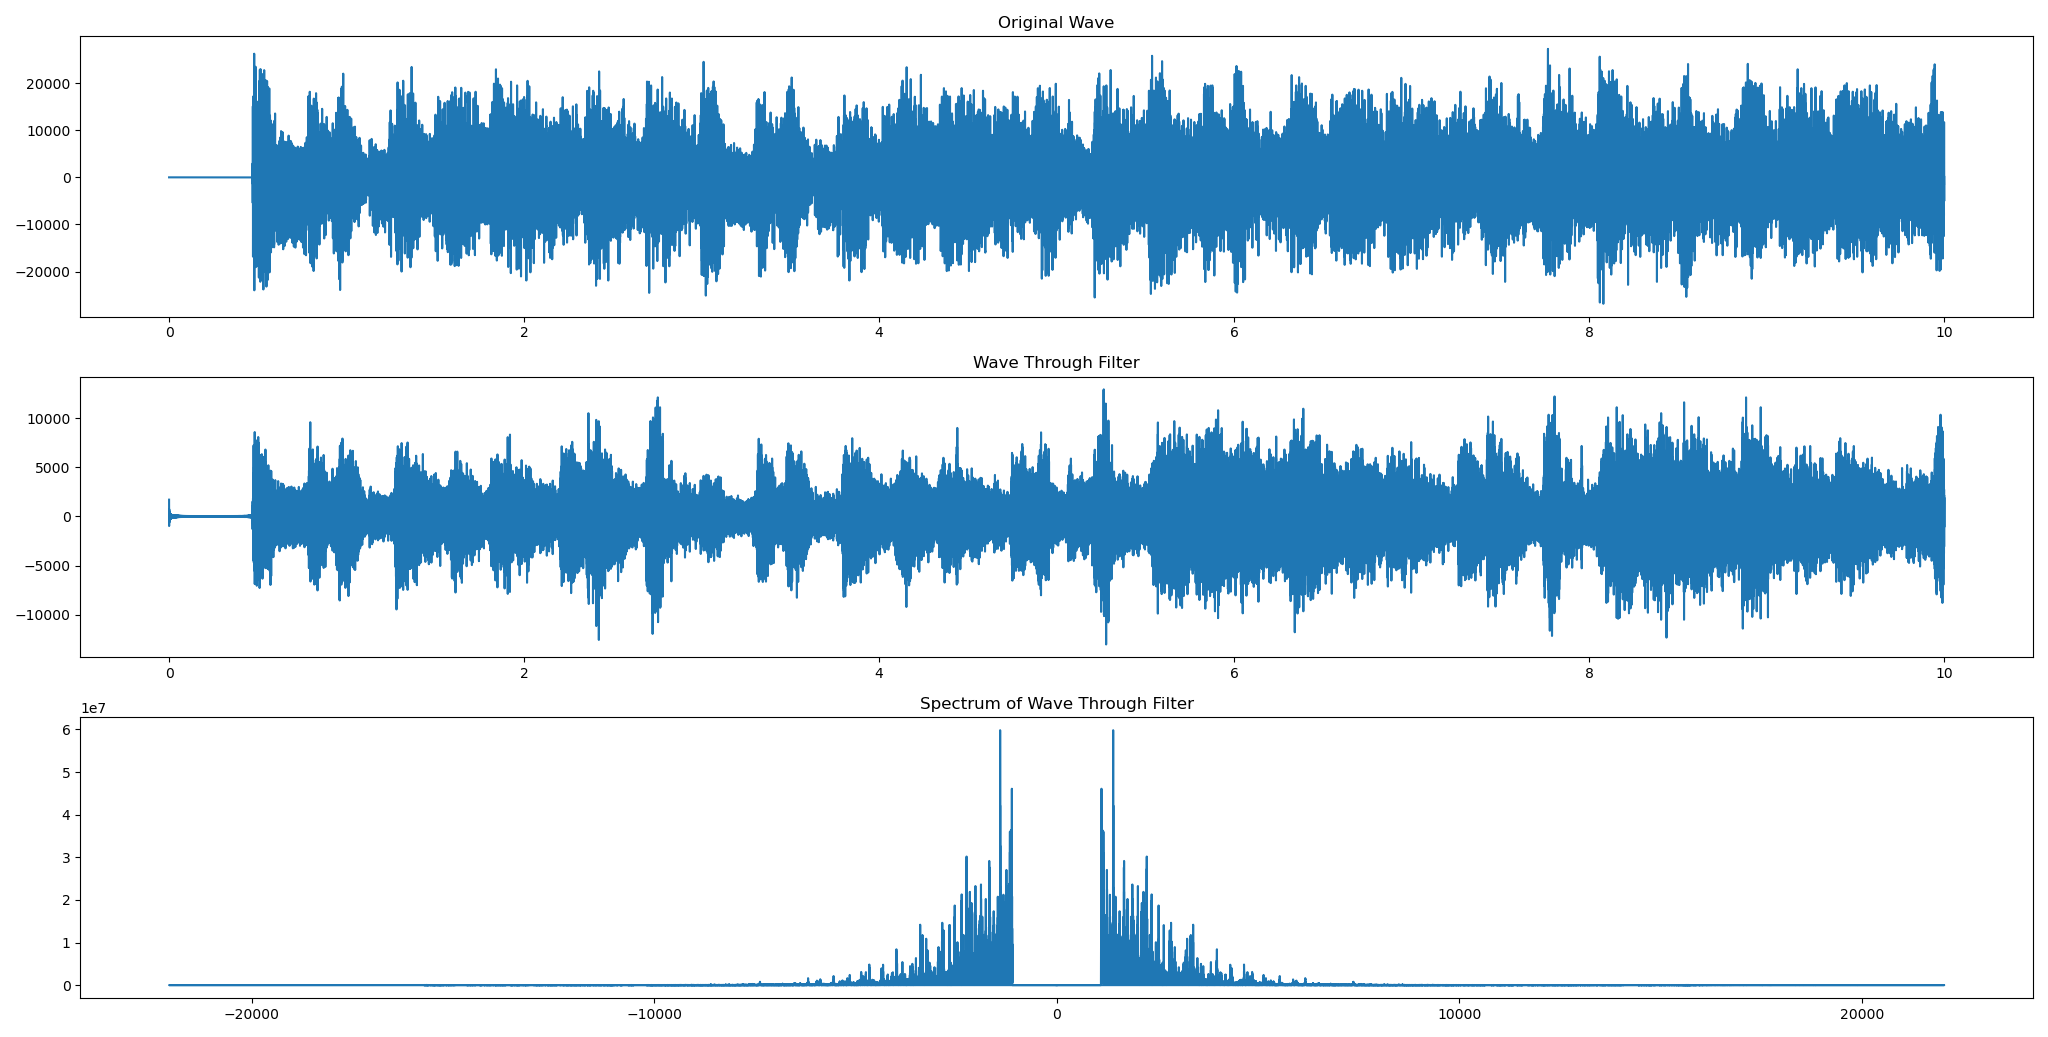
\includegraphics[width=6 in]{../pic/voiceSpectrum.png}
	\caption{Spectrum of My Voice}
	\label{fig:voiceSpectrum}
\end{figure}
\section{Which Contains More Image Information, Amplitude or Phase?}


\bibliographystyle{ieeetr}
\bibliography{../bib/database}

\begin{appendices}
\section{Code Listing}
\begin{python}
import numpy as np
from numpy.fft import fft, fftfreq, ifft
from matplotlib import pyplot as plt
from scipy.io.wavfile import write, read

"""Read Record File"""
fs, x = read('song.wav')
x = x[:, 0]
sec = x.size/fs
t = np.arange(0, sec, 1/fs)

"""Do FFT"""
xt = fft(x)
ap = np.abs(xt)
phase = np.angle(xt)
freq = fftfreq(x.size, d=(1/fs))

"""Simple High-Pass Filter"""
fc = 1100
ap[int(-fc * sec):] = 0
ap[:int(fc * sec)] = 0
"""Simple Low-Pass Filter"""
# cfq = xt.size/2
# ap[int(cfq - (fs/2 - 2000) * seconds):int(cfq + (fs/2 - 2000) * seconds)] = 0

"""Do IFFT And Output"""
xt_f = ap * np.exp(1j * phase)
ix = np.real(ifft(xt_f))
write('out.wav', fs, ix)

"""Draw Wave and Spectrum"""
ax0 = plt.subplot(311)
ax0.set_title("Original Wave")
ax0.plot(t, x)

ax1 = plt.subplot(312) 
ax1.set_title("Wave Through Filter")
ax1.plot(t, ix)

ax2 = plt.subplot(313)
ax2.set_title("Spectrum of Wave Through Filter")
ax2.plot(freq, ap)

plt.show()

\end{python}
\end{appendices}

\end{document}